\chapter{Method}
\label{sec:method}

\section{Data Preparation}
Data preparation is a critical phase in the modeling process, especially for a task involving complex and diverse datasets like ours. Our data preparation process is designed to ensure that the data fed into the model is clean, structured, and suitable for effective analysis and modeling. The following sections describe the steps taken to prepare the data for the multimodal product classification task.

\subsection{Text Data Preprocessing}

To pre-process the "designation" and "description" columns, a custom word-processing function was applied. This function removed HTML tags, replaced accented characters with their corresponding unaccented counterparts, removed special characters and converted all characters to lowercase. These preprocessing steps were selected iteratively in parrallel with the evaluation of the text features extraction model. Some preprocessing were surprinsingly not beneficial to the model performance, such as removing stopwords.\\

Then the text was tokenized, to keep a vocabulary size relatively small, we only kept the word that were present in the product designation of the training dataset (train,valid and test mixed up).
Now that we are writing these lines after fusion model training, we think that we should have separate the train, valid and test dataset before tokenizing the text. So we would have kept only the words that were present in the training dataset. We would see in the future why we think it caused some issues, also we should have kept only the words that were the most frequent so the vocabulary size would have decreased much (many word appears only once).\\

The sequences were then padded to a maximum length of 34, it is the maximum number of words in the designation. The transformation applied on the product description was the same as the product designation. Even if the description can be much longer than the designation, we decided to keep the same maximum length for both, so it makes the fusion of the text features easier, and we also remarked by reading the description in the dataset that longer description were not necessarily more informative. Sometimes, the end of the description was just general information about the seller.\\

\subsection{Image Data Preprocessing}

we remarked that many images were zero padded with a white background, so we decided to remove the white background of the images. We applied a model to find the smallest bounding box that contains no pixels not white, and then we cropped the image to this bounding box.\\
Then we resized the images to 224x224 pixels, because it is the size of the images that were used to train the Clip model.\\

The image data was then preprocessed using the CLIP model's built-in image preprocessing function, we did not do any  other research on the image preprocessing, because we thought that the Clip model would have a good preprocessing function.\\


\subsection{Categorical Encoding of Labels}

In our multimodal product classification task, the target variable 'prdtypecode' represents the category to which each product belongs. This variable is inherently categorical, meaning it represents discrete, non-numeric categories. Each unique 'prdtypecode' corresponds to a different type of product.

Categorical Encoding is used because each 'prdtypecode' is a distinct category with no inherent numerical relationship or order between them. Categorical encoding ensures that the model treats these categories as separate and distinct without assuming any numerical relationship or hierarchy among them \cite{potdar-2017}. If left as is, the model might misinterpret the categorical codes as ordinal or interval  data, leading to incorrect assumptions about the proximity or similarity between different categories.

For this use case One-Hot encoding was used. It converts the categorical target variable into a binary matrix. In this matrix, each category is represented by a vector where only one element is '1', and the rest are '0' \cite{cerda-2018}. This representation avoids any notion of order or magnitude among categories, which is essential for unbiased classification.
With one-hot encoding, no category is given undue preference. For instance, if numeric labels were used directly, the model might assume that higher numbers have more significance or weight, which is not the case in categorical classification.
While one-hot encoding is beneficial, it does increase the dimensionality of the dataset. Each unique category becomes a new feature in the dataset. In cases with many categories, this can lead to a large increase in the number of input features, potentially causing issues like the "curse of dimensionality"\cite{altman-2018}. However, in our context, the benefits of clear and distinct categorical representation outweigh these concerns.

% \section{Visualisation}

\section{Feature Extraction}

\subsection{Image Feature Extraction}

Central to our approach is the integration of OpenAI's CLIP (Contrastive Language–Image Pretraining) model. CLIP is a foundation model based on a transformers and Vit architecture to extract text and image features in the same embedding space.


\begin{figure}[H]
    \centering
    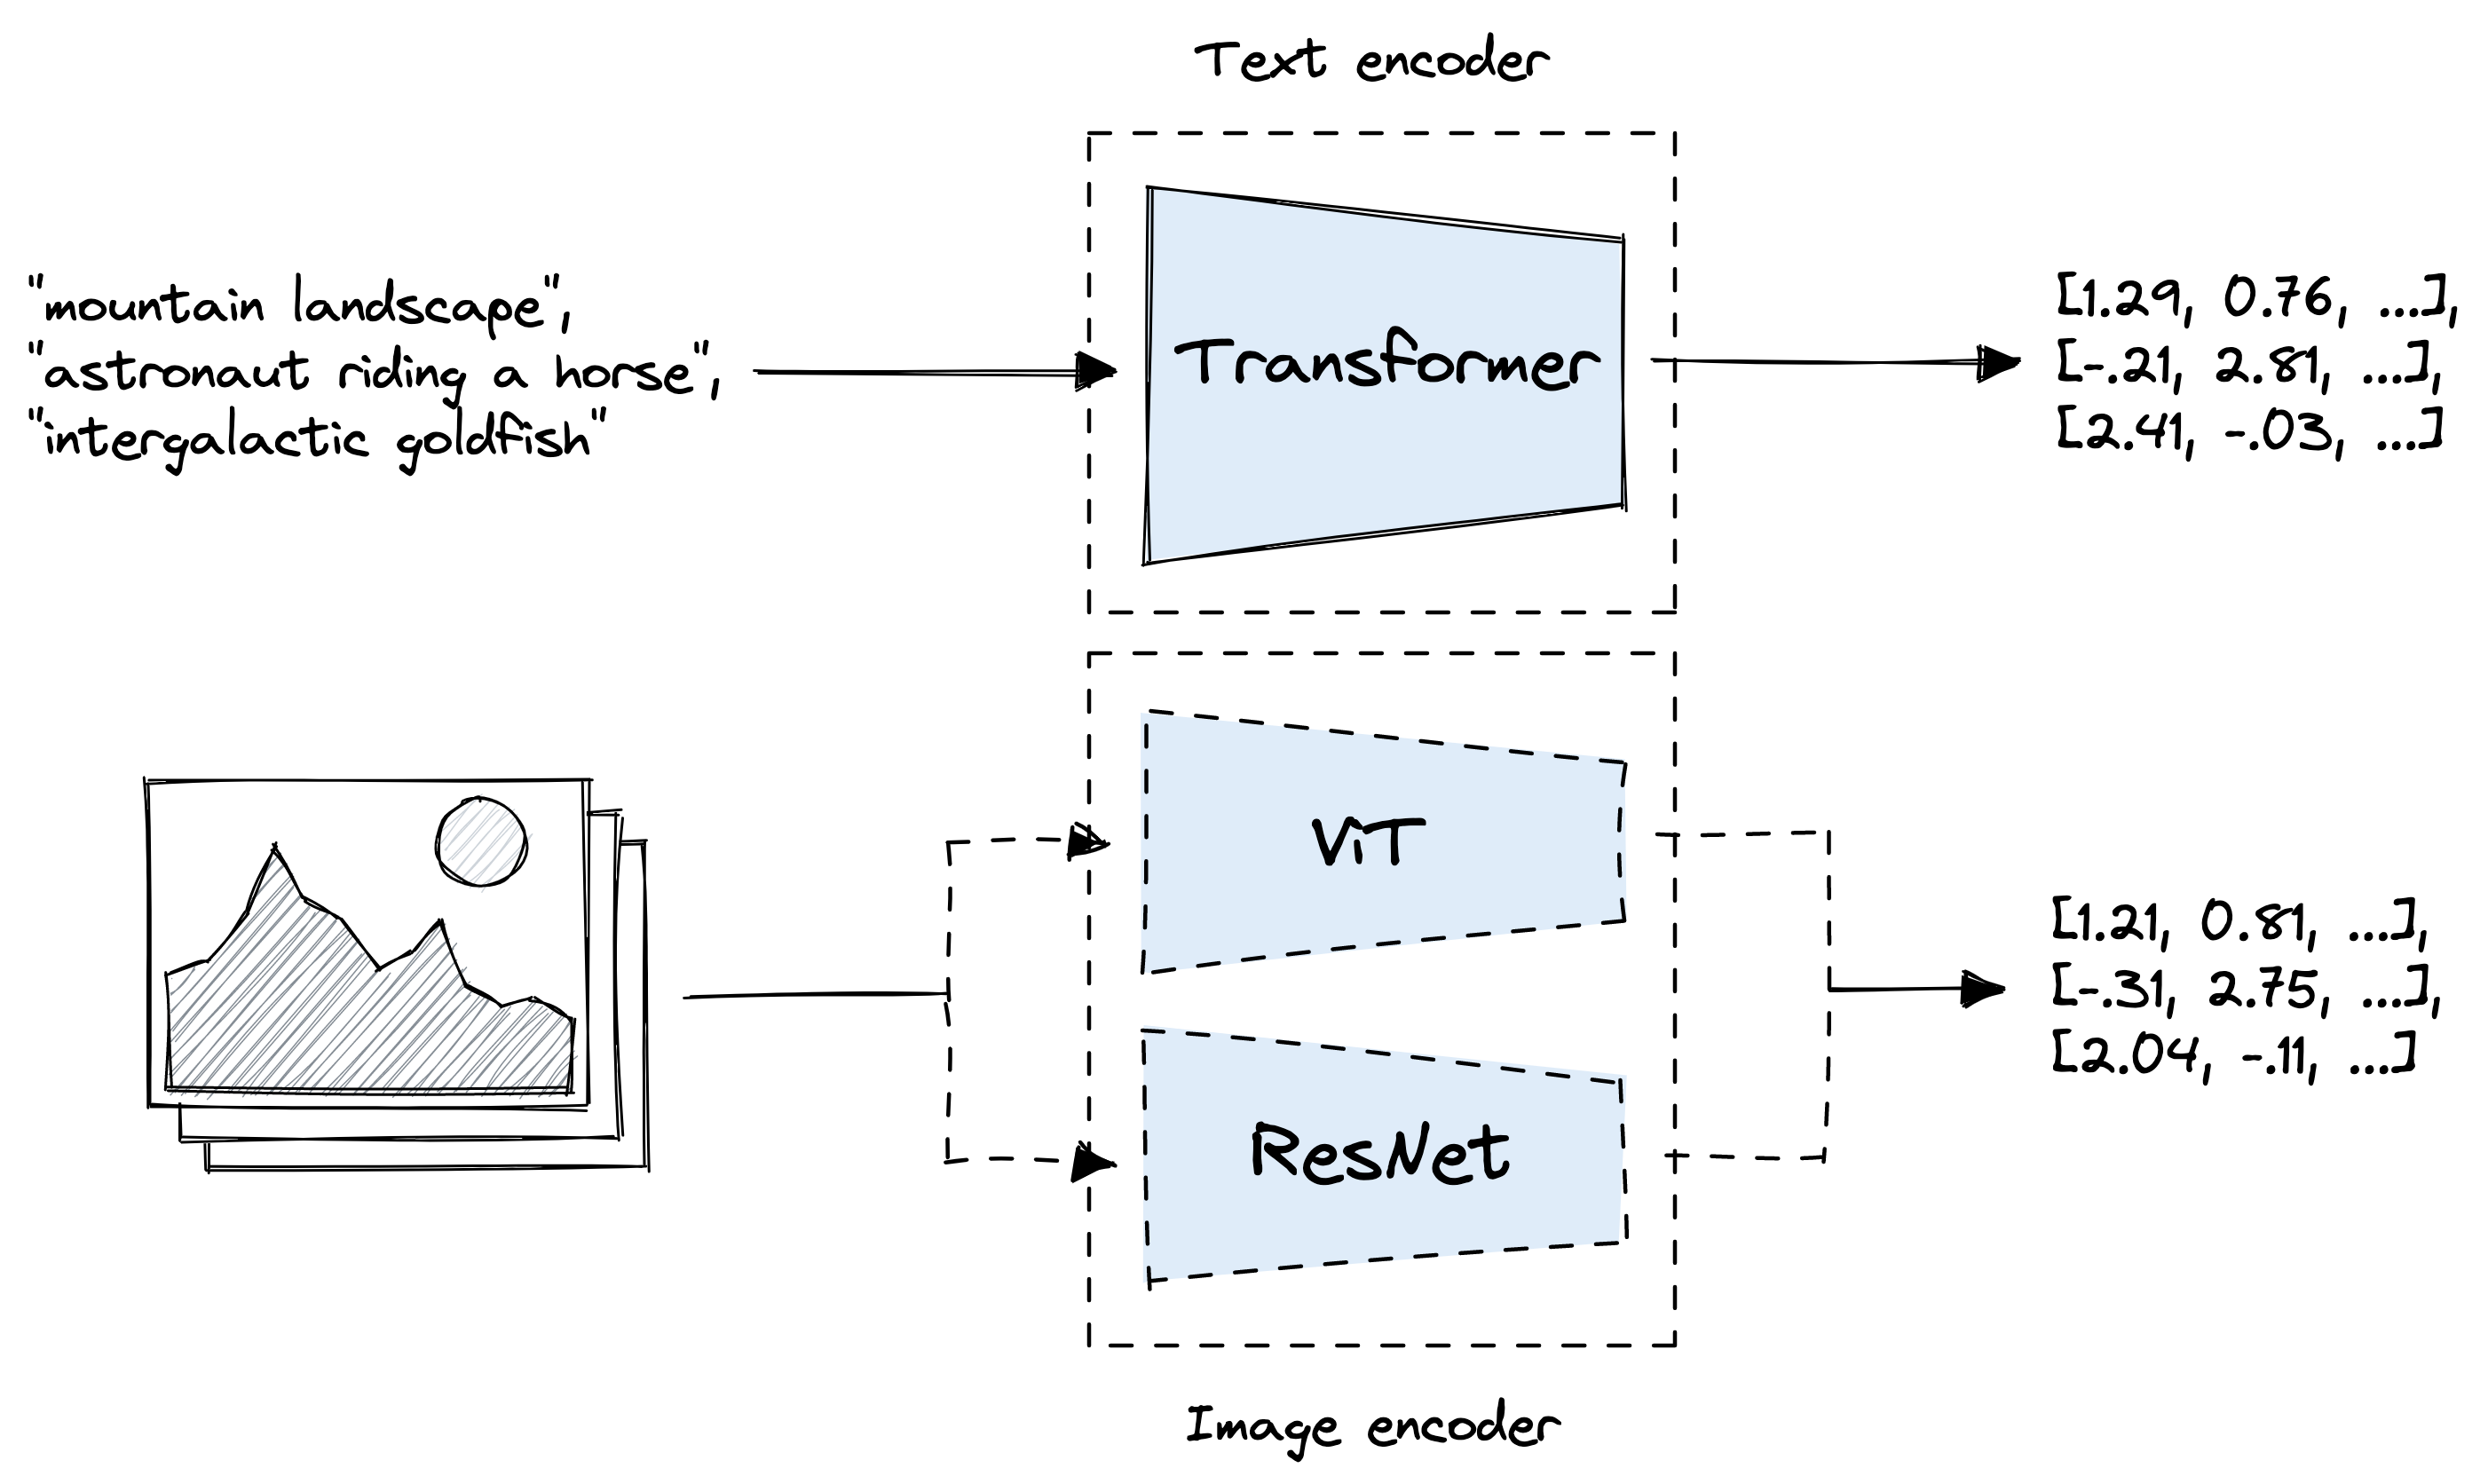
\includegraphics[width=\textwidth]{clip_description.png}
    \caption{\label{fig:clip-architecture}Clip Model presentation}
\end{figure}


As can be seen in the figure \ref{fig:clip-architecture}, CLIP operates on a dual-encoder structure, comprising an image encoder and a text encoder. This architecture is instrumental in processing and correlating visual and textual inputs. The model's training utilizes a contrastive learning method, where it is exposed to numerous images and their corresponding textual descriptions, drawing from a diverse and extensive internet-sourced dataset. This training enables CLIP to develop a nuanced understanding of the intricate relationships between text and images \cite{radford-2021}.
For our use case, We are going to use only the image feature extraction part of the Clip Model, hoping that the image feature extraction done by the clip encoder will provide embeddings that will be separable by the classifier.




\subsection{Textual Feature Extraction}

For the extraction of the features we used a classification model, we used CNN classifier trained both on the designation (product titles) and the non null description fields. The input size is the maximum possible designation length, 34 in this case. Shorter inputs are zero-padded. The architecture consists of an embedding layer and 6 convolutional (with ReLu), max-pooling blocks. The embeddings are trained with the entire architecture. The model architecture can be seen in the figure \ref{fig:text-model}

\begin{figure}[H]
    \centering
    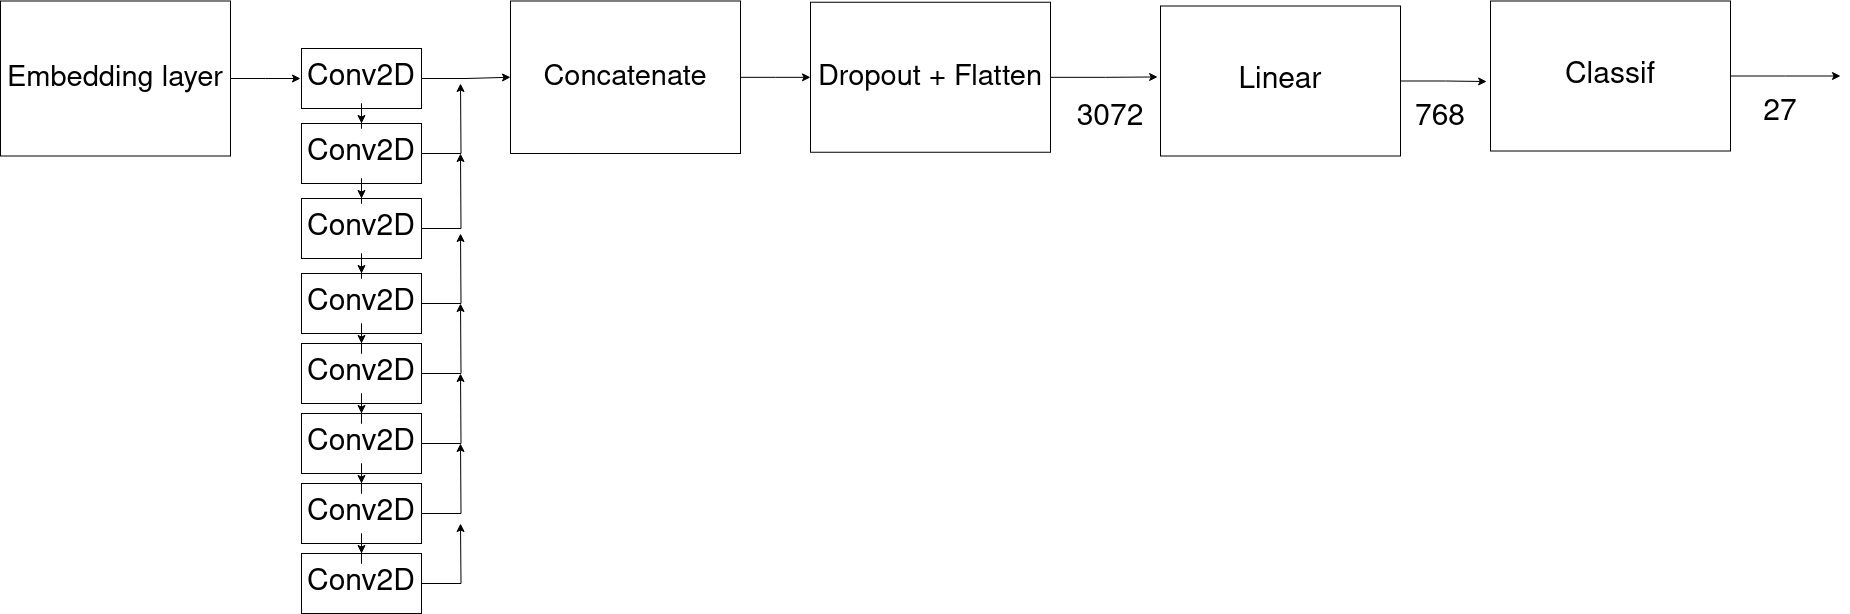
\includegraphics[width=\textwidth]{text-model-architecture.png}
    \caption{Text Model Architecture}
    \label{fig:text-model}
\end{figure}


We succeeded reaching a 0.747 weighted F1-score on the test dataset of the challenge. After the training of this model, we extracted the embeddings of the last linear layer. The embeddings are of size 768, wich match the size of the CLIP embeddings. We then used these embeddings as input for the multimodal model.

\subsection{Features Fusion}

\begin{figure}[H]
    \centering
    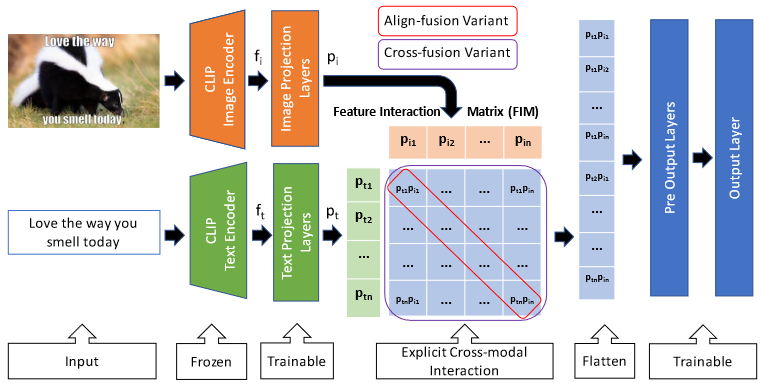
\includegraphics[width=\textwidth]{hateclip.png}
    \caption{\label{fig:hateclipper} Proposed architecture of Hate-CLIPper for Multimodal Hateful Meme Classification}

\end{figure}

At the core of our feature extraction process lies the Feature Interaction Matrix (FIM),wich is obtained by calculating the product between the image features anf the text features, the obtained matrices captures the intricate relationships between textual and visual features (see Figure \ref{fig:hateclipper}). This approach, as outlined in the "Hate-CLIPper" paper \cite{kumar2022hateclipper}, effectively harnesses the strengths of CLIP's robust feature extraction capabilities while expanding its ability to discern the intricate associations that simpler models might overlook. The FIM consequently enables a more holistic and contextually aware representation of the data, augmenting the model's capacity for accurate classification in complex multimodal tasks.

\section{Classification}

After flattening  the FIM, we used a simple 2 layer linear classifier to predict the prdtypecode. The classifier is a simple linear layer . The model is trained with the cross entropy loss function, SGD optimizer with a learning rate of 0.001 and a 0.9 momentum was used, and the model was trained with a batch size of 128.

It takes approximately 4 hours per epoch to train the model on a A 200 GPU . According to our observation the first epoch is a really good observation of what we would expect with longer training.

The time that takes the model to be trained is mostly due to the Clip model wich is an expensive transformers architecture. We could also have used a projection layer from the Clip features to an embedding layer the same as the text features, but we did not have time to try it.

As the variety of product is quite large, we think that it is interesting to use a foundation model that already seen a lot of unique products, and that is why we chose to use the Clip model. We think that the model could have been improved by using a model that is trained on a dataset that is more similar to the one we are using, but we did found one.

\begin{figure}[H]
    \centering
    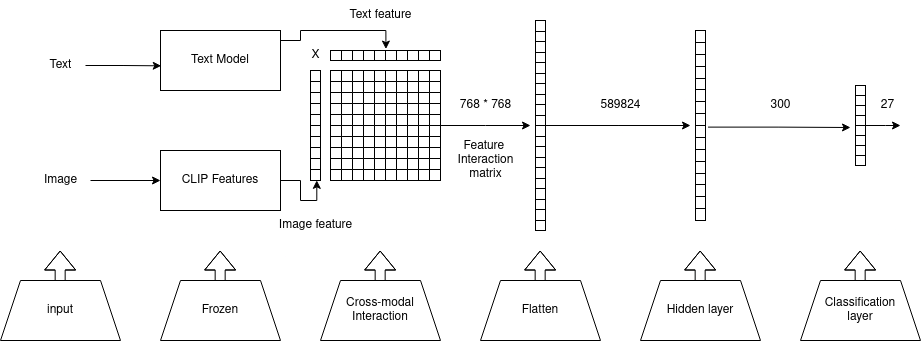
\includegraphics[width=\textwidth]{model.png}
    \caption{Architecture of our multimodal model}
    \label{fig:model}
\end{figure}